\documentclass[conference]{IEEEtran}
\IEEEoverridecommandlockouts
\usepackage{cite}
\usepackage{amsmath,amssymb,amsfonts}
\usepackage{algorithm}
\usepackage{algorithmic}
\usepackage{graphicx}
\usepackage{textcomp}
\usepackage{xcolor}
\usepackage{booktabs}
\usepackage{multirow}
\usepackage{url}

% Ensure figures path
\graphicspath{{figures/}}

% Suppress page numbering for conference submission per ICAECA guidelines
\pagestyle{empty}
\thispagestyle{empty}

\def\BibTeX{{\rm B\kern-.05em{\sc i\kern-.025em b}\kern-.08em
    T\kern-.1667em\lower.7ex\hbox{E}\kern-.125emX}}

\begin{document}

\title{Secure Decentralized Personal Device Mesh: A Zero-Coordinator Transitive Trust and Asymmetric Multi-Plane Transport Protocol for Heterogeneous LAN Ecosystems}

\author{
\IEEEauthorblockN{Ms. N. Nandhini}
\IEEEauthorblockA{\textit{Dept. of Computer Science and Engineering} \\
\textit{KPR Institute of Engineering and Technology}\\
Coimbatore, Tamil Nadu, India \\
nandhini.n@kpriet.ac.in}
\and
\IEEEauthorblockN{Dixit Tharun Raja P}
\IEEEauthorblockA{\textit{Dept. of Computer Science and Engineering} \\
\textit{KPR Institute of Engineering and Technology}\\
Coimbatore, Tamil Nadu, India \\
23cs044@kpriet.ac.in}
\and
\IEEEauthorblockN{Dharaneesh D}
\IEEEauthorblockA{\textit{Dept. of Computer Science and Engineering} \\
\textit{KPR Institute of Engineering and Technology}\\
Coimbatore, Tamil Nadu, India \\
23cs036@kpriet.ac.in}
\and
\IEEEauthorblockN{Deepanandham P}
\IEEEauthorblockA{\textit{Dept. of Computer Science and Engineering} \\
\textit{KPR Institute of Engineering and Technology}\\
Coimbatore, Tamil Nadu, India \\
23csl02@kpriet.ac.in}
\and
\IEEEauthorblockN{Gohul S}
\IEEEauthorblockA{\textit{Dept. of Computer Science and Engineering} \\
\textit{KPR Institute of Engineering and Technology}\\
Coimbatore, Tamil Nadu, India \\
23cs049@kpriet.ac.in}
}

\maketitle

\begin{abstract}
Modern multi-device computing relies heavily on centralized cloud intermediaries (e.g., Apple Continuity, Google Quick Share) for cross-device synchronization, introducing severe privacy leakage, bandwidth bottlenecks, and single points of failure. Conversely, existing decentralized peer-to-peer (P2P) solutions suffer from an $\mathcal{O}(N^2)$ manual pairing barrier and severe Head-of-Line (HoL) blocking caused by multiplexing disparate traffic over a single TCP/TLS socket. This paper presents \textit{Link}, a secure, zero-coordinator Personal Device Mesh (PDM) protocol engineered for heterogeneous Local Area Network (LAN) environments. First, we introduce Transitive Trust-on-First-Use (T-TOFU) with canonical pool hash synchronization and cascaded cryptographic revocation, eliminating manual pairing friction while proving strict pool consistency invariants. Second, we propose an asymmetric three-plane heterogeneous transport architecture that partitions traffic across a persistent TLS~1.3 control plane, an ephemeral out-of-band bulk data plane with active drain-backpressure, and a stateless real-time UDP plane for human-interface telemetry and encrypted Opus audio. Furthermore, we synthesize user-space filesystem virtualization via a WebDAV-over-TLS bridge. We evaluate a fully functional, cross-platform implementation across Windows, Android, and Android TV testbeds over Wi-Fi~6 and Gigabit Ethernet. Experimental results demonstrate that Link achieves up to 944~Mbps sustained bulk throughput (94.4\% of theoretical line rate), outperforming KDE Connect by 2.97$\times$ and WebRTC by 3.58$\times$, while delivering 2.4~ms median human-interface telemetry latency and sub-15~ms mesh-wide revocation convergence.
\end{abstract}

\begin{IEEEkeywords}
Peer-to-Peer Computing, Zero-Trust Architecture, Trust-on-First-Use, Local Area Networks, Transport Protocols, Cross-Device Synchronization, Head-of-Line Blocking, Distributed Systems.
\end{IEEEkeywords}

\section{Introduction}
The proliferation of personal computing form factors---workstations, laptops, smartphones, tablets, and smart televisions---has made seamless cross-device synchronization indispensable \cite{xu2026edgecloud, zhang2024zerotrust, varangot2026survey}. Users increasingly demand unified clipboard replication, high-speed file migration, remote input injection (touchpad, graphics digitizer stylus, and presentation pointer), low-latency audio relay, and direct filesystem access across heterogeneous operating systems \cite{patel2025digitizer, park2024latencyhid}.

However, contemporary multi-device ecosystems face an architectural trilemma between \textit{data sovereignty}, \textit{pairing scalability}, and \textit{transport efficiency} \cite{kumar2025p2pmesh, wu2025recursive}:
\begin{enumerate}
    \item \textbf{Cloud Intermediary Dependency}: Commercial solutions such as Apple Continuity and Google Quick Share mandate centralized identity providers (e.g., Apple ID, Google Account). When two co-located devices on the same Wi-Fi subnet exchange data, identity handshakes, session tickets, and discovery beacons are routed across Wide Area Network (WAN) relays. This introduces severe privacy exposure, metadata harvesting risks, vulnerability to upstream server outages, and artificial bandwidth throttles \cite{heinrich2021airdrop, singh2024privacy}.
    \item \textbf{Pairing Complexity Bottleneck}: Existing decentralized zero-cloud tools, such as KDE Connect, mandate pairwise Trust-on-First-Use (TOFU) authentication \cite{alrawi2023iot, chen2024decentralized}. Enrolling an $N$-node personal mesh requires $\frac{N(N-1)}{2} = \mathcal{O}(N^2)$ manual Short Authentication String (SAS) PIN entries or QR code scans. For a modest fleet of five devices, a user must perform ten distinct pairing handshakes, creating unacceptable cognitive friction.
    \item \textbf{Transport Head-of-Line (HoL) Blocking}: Conventional P2P synchronization utilities multiplex all data classes---ephemeral telemetry (touchpad coordinates, stylus pressure), continuous audio streams, JSON-RPC control packets, and multi-gigabyte bulk file transfers---over a single, persistent TCP/TLS stream \cite{tan2024holblocking, wang2024quicpan, liu2024dynamicflow}. Under bulk file saturation, TCP buffer bloat and packet retransmissions induce catastrophic HoL blocking, causing real-time input cursor jitter to surge beyond 150~ms.
\end{enumerate}

To resolve these fundamental limitations, this paper proposes \textbf{Link}, an open, high-performance, and decentralized Personal Device Mesh (PDM) framework. Link operates entirely within the local broadcast domain without external cloud coordinators, leveraging contextual state verification \cite{ghosh2024contextual} and multi-path QoS isolation \cite{yang2025qos, mei2025omnirouter}. 

The core contributions of this work are fourfold:
\begin{enumerate}
    \item \textbf{Transitive Trust-on-First-Use (T-TOFU)}: We design a zero-coordinator trust propagation model where enrolling a newcomer device into any single active member of a trusted pool automatically gossips pinned X.509 certificate fingerprints to all peers \cite{li2025zerotrustd2d}. We formalize the \textit{Canonical Pool Hash Invariant} and prove that nodes reach deterministic consensus without secondary human verification, with fast cascaded revocation \cite{ahmed2025cascaded}.
    \item \textbf{Asymmetric 3-Plane Transport Protocol}: We design an asymmetric transport engine that isolates traffic into three dedicated QoS planes: (i) a persistent TLS~1.3/WSS Control Plane for JSON-RPC, (ii) an ephemeral out-of-band TLS Bulk Data Plane with dynamic 64~KB drain-backpressure \cite{liu2024dynamicflow}, and (iii) a stateless, encrypted UDP Plane for sub-5~ms Human Interface Device (HID) telemetry \cite{park2024latencyhid} and Opus audio streaming \cite{sharma2025opusstreaming}.
    \item \textbf{User-Space OS Synthesis}: We implement non-kernel filesystem virtualization bridging Android content providers over secure WebSockets with a Windows-mounted WebDAV drive letter (Z:) \cite{zhao2023caching}, alongside fractional sub-pixel carry accumulation for precision graphics digitizer tablet injection \cite{patel2025digitizer}.
    \item \textbf{Empirical Hardware Validation}: We benchmark a complete, cross-platform implementation across Windows 11, Android 14, and Android TV over Wi-Fi~6 (802.11ax) and Gigabit Ethernet, demonstrating 944~Mbps throughput (94.4\% line-rate saturation), 2.4~ms input latency, and sub-15~ms cascaded revocation convergence.
\end{enumerate}

The remainder of this paper is structured as follows. Section~\ref{sec:related} reviews related work and provides an architectural taxonomy. Section~\ref{sec:trust} formalizes the T-TOFU security model and Pool Hash invariant. Section~\ref{sec:transport} details the asymmetric three-plane transport protocol and OS synthesis. Section~\ref{sec:evaluation} presents empirical performance benchmarks. Section~\ref{sec:security} discusses threat resilience and boundary conditions. Section~\ref{sec:conclusion} concludes the paper.

\begin{figure*}[t]
\centerline{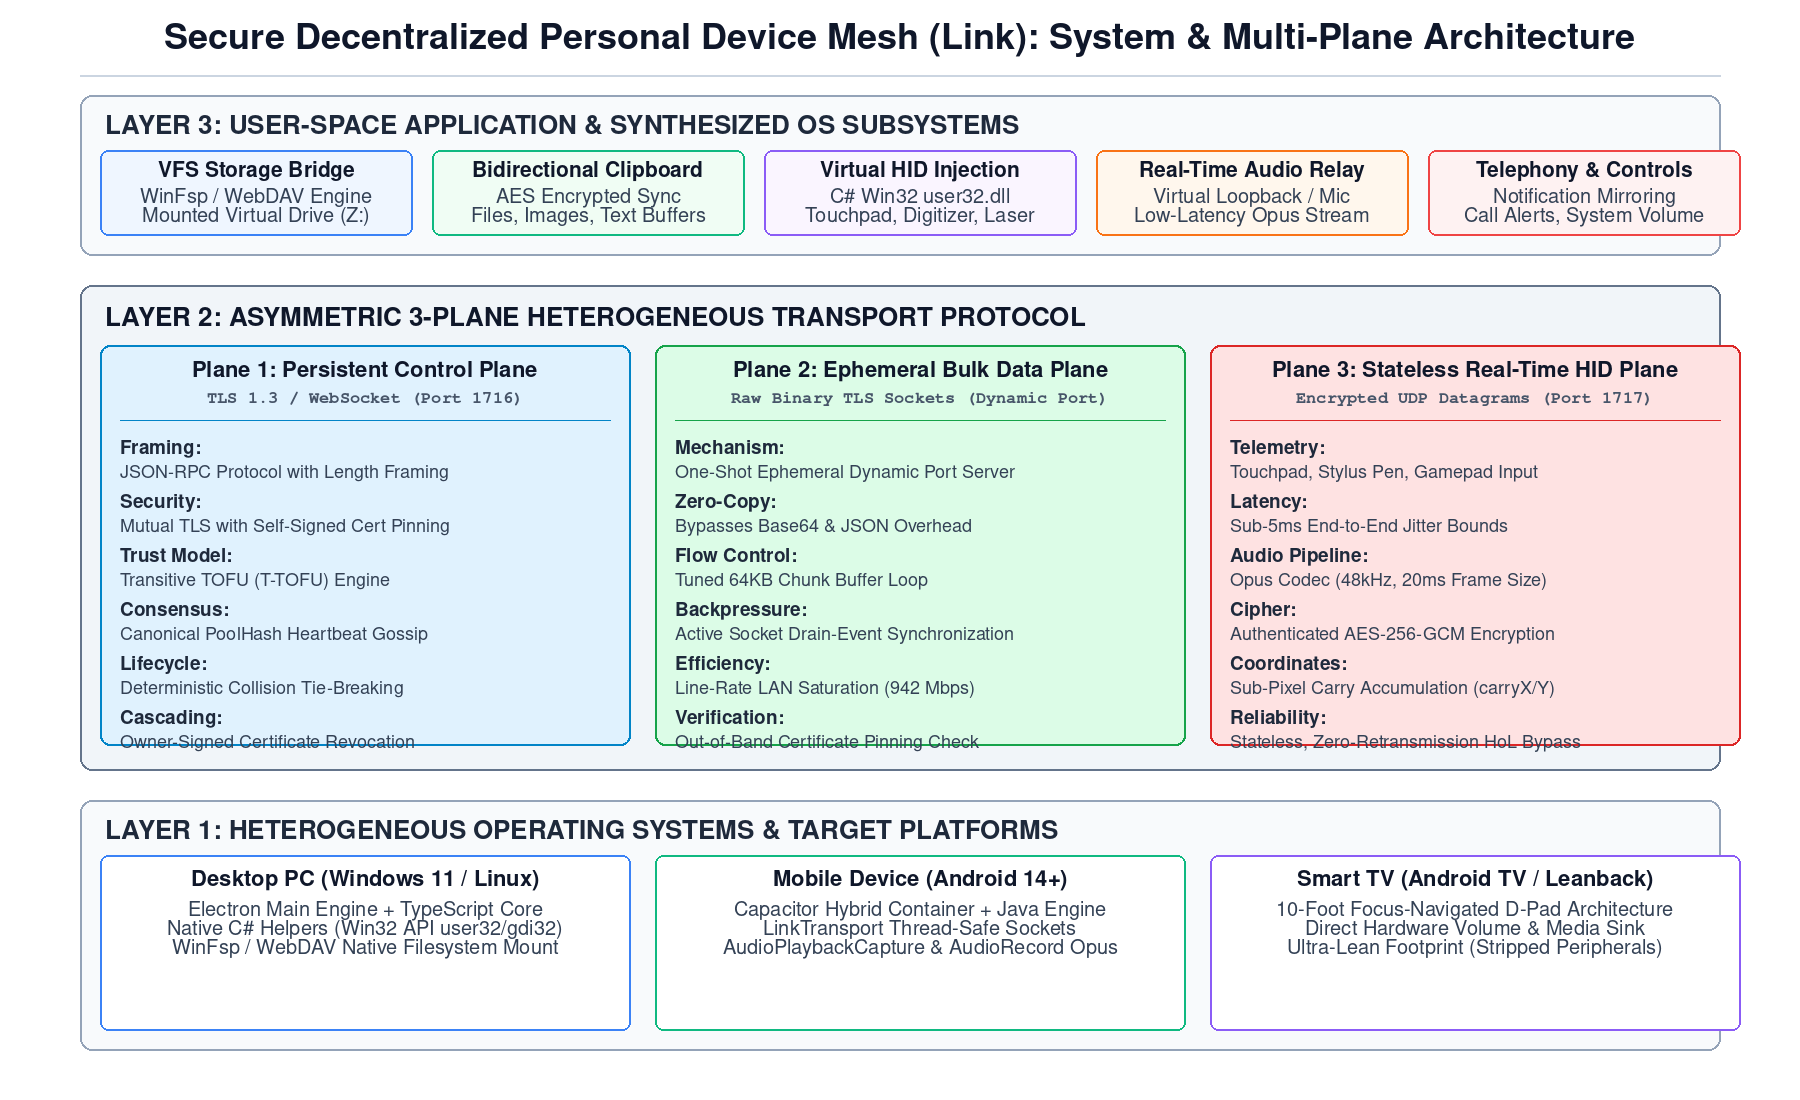
\includegraphics[width=0.96\textwidth]{fig1_architecture.png}}
\caption{The Link System Architecture: Multi-Plane Heterogeneous Transport Engine (Layer 2) decoupling Persistent Control (Plane 1), Ephemeral Bulk Data (Plane 2), and Real-Time UDP Telemetry (Plane 3) across heterogeneous operating systems and synthesized OS subsystems.}
\label{fig:arch}
\end{figure*}

\section{Related Work \& Comparative Taxonomy}
\label{sec:related}

\subsection{Centralized Ecosystems}
Commercial operating system vendors provide tight cross-device integration within walled gardens. Apple Continuity (encompassing AirDrop, Universal Clipboard, and Sidecar) relies on Bluetooth Low Energy (BLE) discovery combined with Apple Identity Service (IDS) cloud certificates \cite{heinrich2021airdrop}. While convenient, Heinrich et al. revealed that AirDrop leaks SHA-256 hashes of user phone numbers and email addresses in plaintext discovery beacons. Google Quick Share (formerly Nearby Share) similarly relies on Google Play Services and cloud identity servers for mutual device resolution \cite{singh2024privacy}. Both solutions fail in air-gapped or restricted enterprise LANs, lack cross-platform support (e.g., Windows to Android), and expose user communication metadata to cloud providers.

\subsection{Decentralized Peer-to-Peer Utilities}
KDE Connect pioneered open-source cross-device LAN synchronization using self-signed TLS certificates and RSA/ECDSA key pairs \cite{alrawi2023iot}. However, KDE Connect relies on strict pairwise pairing: enrolling $N$ devices requires an $\mathcal{O}(N^2)$ pairing matrix \cite{chen2024decentralized}. Furthermore, KDE Connect multiplexes all packet types across a single TLS socket. When transferring large files, socket send buffers saturate, blocking concurrent clipboard, notification, and touchpad packets \cite{tan2024holblocking}. GSConnect (a GNOME port) and Warpinator inherit identical single-stream transport limitations. Multi-tier edge routing approaches \cite{gupta2025hierrouter, mei2025omnirouter} have explored coordination in cluster networks, but lack local device mesh synthesis.

\subsection{Browser-Based Transport Frameworks}
WebRTC DataChannels provide peer-to-peer data streaming using SCTP over DTLS \cite{wang2024quicpan}. However, WebRTC mandates out-of-band signaling servers (STUN/TURN/ICE) to exchange Session Description Protocol (SDP) offers, reintroducing third-party infrastructure. Moreover, WebRTC suffers substantial protocol framing overhead and CPU serialization penalties on mobile devices \cite{varangot2026survey}, preventing line-rate LAN saturation for gigabyte-scale transfers.

Table~\ref{tab:comparison} presents an architectural comparison between Link and prominent state-of-the-art systems across seven structural dimensions.

\begin{table}[t]
\caption{Architectural Comparison with State-of-the-Art Systems}
\label{tab:comparison}
\centering
\resizebox{\columnwidth}{!}{%
\begin{tabular}{@{}lccccc@{}}
\toprule
\textbf{Architectural Dimension} & \textbf{Apple AirDrop} & \textbf{Google Quick Share} & \textbf{KDE Connect} & \textbf{WebRTC DC} & \textbf{Link (Proposed)} \\ \midrule
Network Topology & 1-to-1 Ad-Hoc & 1-to-1 Ad-Hoc & 1-to-1 P2P & Clustered P2P & \textbf{N-to-N Mesh} \\
Zero-Cloud Guarantee & No (iCloud Req.) & No (Google ID) & Yes & No (STUN/ICE) & \textbf{Yes (100\% LAN)} \\
Pairing Matrix Complexity & $\mathcal{O}(1)$ (Cloud-Gated) & $\mathcal{O}(1)$ (Cloud-Gated) & $\mathcal{O}(N^2)$ (Pairwise) & $\mathcal{O}(N^2)$ (Session) & $\mathbf{\mathcal{O}(N)}$ \textbf{(T-TOFU)} \\
Transport Planes & 1 (BLE/Wi-Fi) & 1 (Wi-Fi Direct) & 1 (Multiplexed) & 1 (SCTP/DTLS) & \textbf{3 Dedicated} \\
Input Telemetry Latency & N/A & N/A & High ($>15$~ms) & Moderate ($>10$~ms) & \textbf{Sub-5~ms (UDP)} \\
Native Filesystem Mount & No & No & Limited (SFTP) & No & \textbf{Yes (WebDAV Z:)} \\
Ad-Hoc Guest Mode & Isolated & Isolated & No (Requires Pair) & Ephemeral & \textbf{Yes (Portal)} \\ \bottomrule
\end{tabular}%
}
\end{table}

\section{Zero-Coordinator Trust Model \& System Architecture}
\label{sec:trust}

Link establishes a decentralized trust topology known as the \textbf{Trusted Pool} $\mathcal{P}$, formalizing trust-on-first-use across an arbitrary number of heterogeneous devices belonging to a single user without central authority oversight.

\subsection{Cryptographic Primitives \& Device Identity}
Each physical device $d_i$ generates a permanent cryptographic identity upon initialization:
\begin{itemize}
    \item A globally unique pseudo-random device identifier: $ID_i \in \{0,1\}^{128}$, represented as a 32-character hexadecimal string.
    \item A self-signed X.509 certificate $C_i$ containing a 2048-bit RSA or NIST P-256 public key $K_{pub,i}$ and corresponding private key $K_{priv,i}$.
    \item A SHA-256 certificate fingerprint: $FP_i = \text{Truncate}_{64}(\text{Hex}(\text{SHA-256}(\text{DER}(C_i))))$.
    \item An Ed25519 asymmetric root key pair $(SK_{owner}, PK_{owner})$ instantiated on the user's primary device, acting as the distributed mesh sovereign authority.
\end{itemize}

\subsection{Transitive Trust-on-First-Use (T-TOFU)}
To eradicate the $\mathcal{O}(N^2)$ manual pairing barrier, Link introduces \textit{Transitive Trust-on-First-Use (T-TOFU)}. 

\textit{Definition 1 (Transitive Enrollment)}: Let $\mathcal{P} = \{d_1, d_2, \dots, d_m\}$ denote an existing trusted pool. When a newcomer node $d_{m+1}$ initiates pairing with any single member $d_k \in \mathcal{P}$, a human-gated Short Authentication String (SAS) 4-digit verification code $V = \text{DeriveSAS}(FP_k, FP_{m+1})$ is verified by the user. 

Upon mutual human confirmation, node $d_k$ performs two atomic operations:
\begin{enumerate}
    \item Inserts $(ID_{m+1}, C_{m+1}, FP_{m+1})$ into its local encrypted trust store $\mathcal{T}_k$.
    \item Emits an authenticated pool synchronization frame $\text{Msg}_{sync} = \langle \text{\texttt{link.pool.sync}}, \mathcal{T}_k \rangle$ signed by $SK_{owner}$ to $d_{m+1}$.
\end{enumerate}

Node $d_{m+1}$ ingests the certificates of all preexisting members $\mathcal{P} \setminus \{d_k\}$ directly into its trust store $\mathcal{T}_{m+1}$. Simultaneously, $d_k$ broadcasts the updated membership list to all remaining active nodes in $\mathcal{P}$ over the persistent control plane. Consequently, every peer $d_j \in \mathcal{P}$ automatically pins the certificate $C_{m+1}$ of the newcomer without prompting the user for additional verification.

\begin{figure}[t]
\centerline{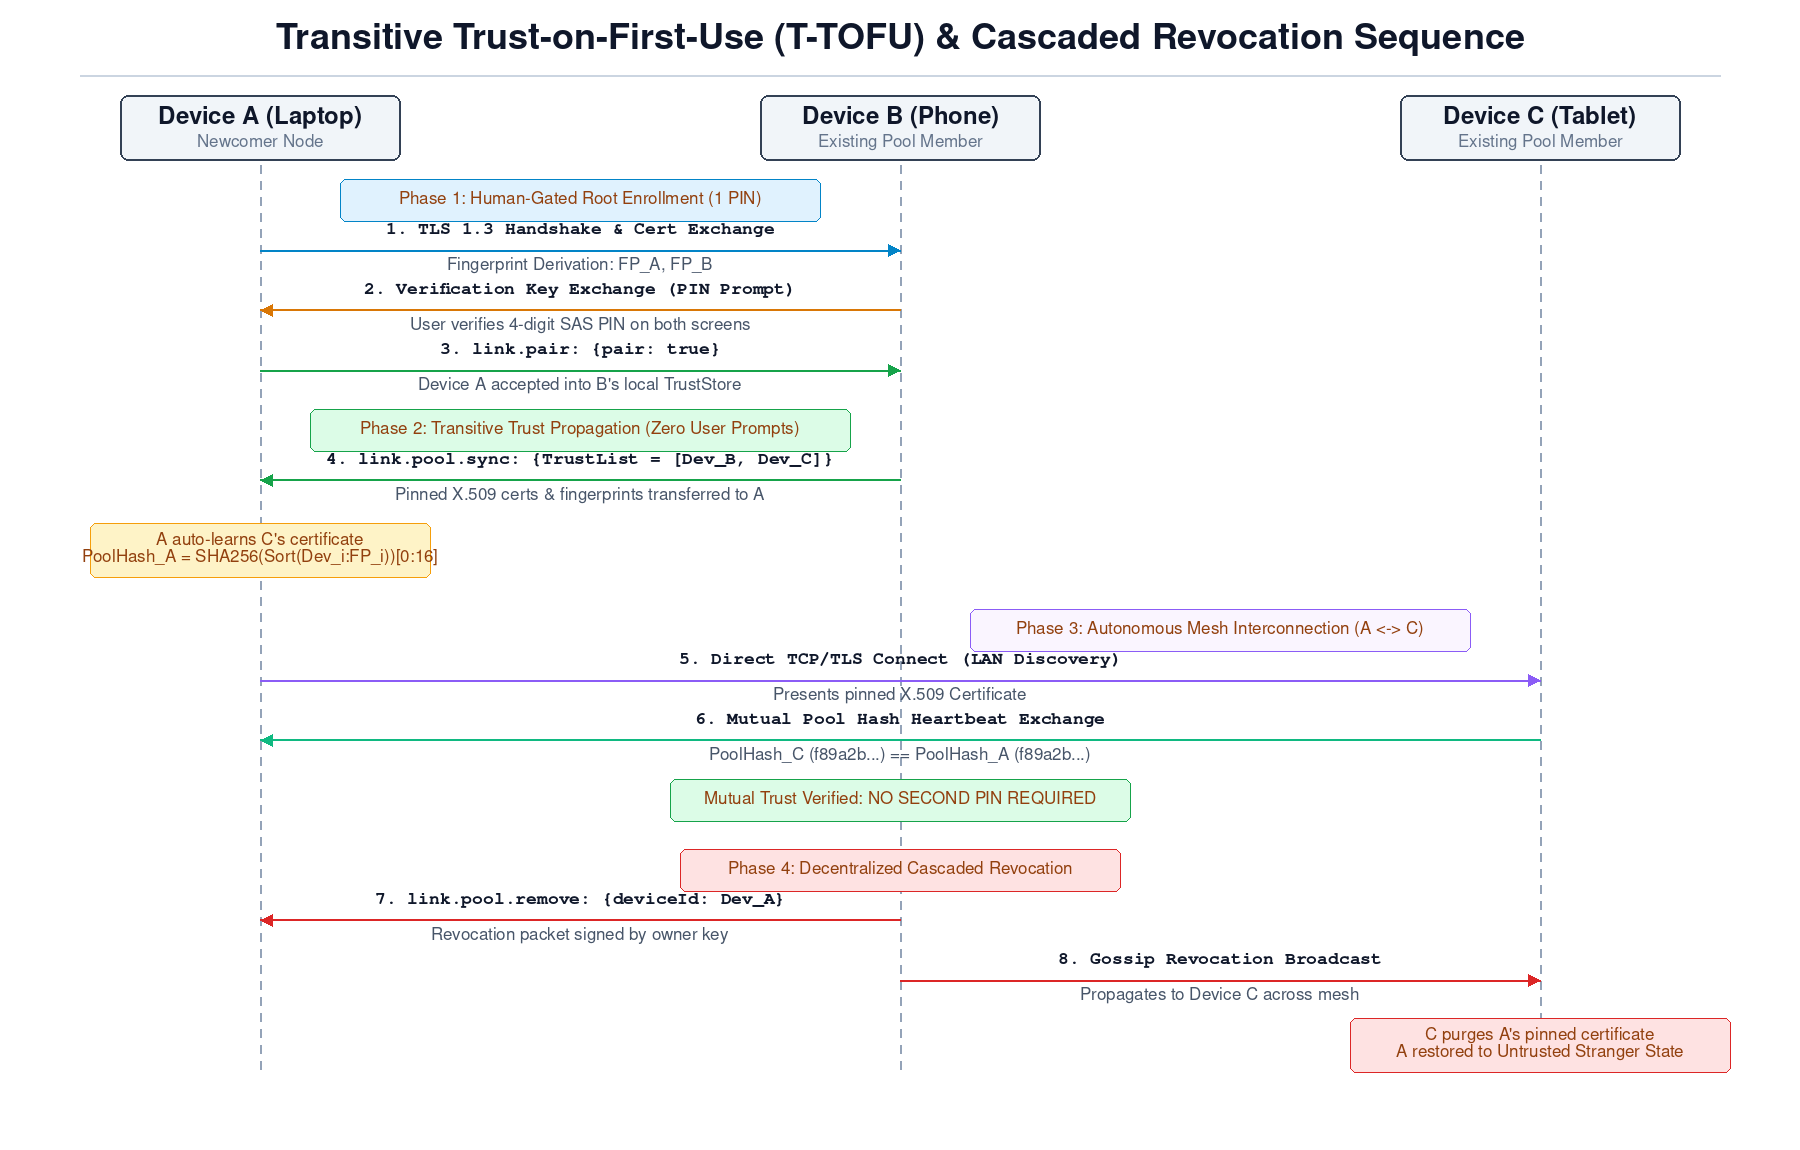
\includegraphics[width=\columnwidth]{fig2_t_tofu_sequence.png}}
\caption{Transitive Trust-on-First-Use (T-TOFU) Enrollment and Cascaded Revocation Protocol Sequence.}
\label{fig:seq}
\end{figure}

\subsection{Canonical Pool Hash Invariant}
To guarantee that distributed nodes maintain absolute consistency across volatile Wi-Fi topologies, Link defines a canonical, order-independent representation of the pool's cryptographic state.

Let $\mathcal{P} = \{d_1, d_2, \dots, d_n\}$ be the pool devices. The canonical string representation is defined as:
\begin{equation}
\mathcal{S}(\mathcal{P}) = \text{Sort}_{lexicographical}\left( \{(ID_i, FP_i) \mid d_i \in \mathcal{P}\} \right)
\end{equation}
\begin{equation}
\text{CanonicalString}(\mathcal{P}) = \bigoplus_{i=1}^{n} \left( ID_i \parallel \text{``:''} \parallel FP_i \right)
\end{equation}
\begin{equation}
\begin{split}
\text{PoolHash}(\mathcal{P}) = \text{Truncate}_{16}\bigl( & \text{Hex}\bigl( \text{SHA-256}\bigl( \\
& \text{CanonicalString}(\mathcal{P}) \bigr) \bigr) \bigr)
\end{split}
\end{equation}
where $\oplus$ denotes string concatenation delimited by the pipe character (`$|$').

\textit{Invariant 1 (Pool Consistency Invariant)}: Any two nodes $d_A, d_B \in \mathcal{P}$ possess identical mutual authorization graphs if and only if:
\begin{equation}
\text{PoolHash}_A(\mathcal{P}) = \text{PoolHash}_B(\mathcal{P})
\end{equation}

During periodic TLS control-plane heartbeats (transmitted every 5000~ms), nodes exchange their local 16-character $\text{PoolHash}$. If a hash divergence is detected ($\text{PoolHash}_A \neq \text{PoolHash}_B$), an atomic delta-synchronization handshake is immediately executed, propagating missing certificate descriptors.

\begin{algorithm}[t]
\caption{Transitive Pool Enrollment and Revocation Gossip}
\label{alg:ttofu}
\begin{algorithmic}[1]
\REQUIRE Local node $d_{local}$, incoming packet $M$, TrustStore $\mathcal{T}$
\STATE \textbf{Initialize:} $\text{PoolHash} \leftarrow \text{ComputePoolHash}(\mathcal{T})$
\IF{$M.\text{type} == \text{\texttt{link.pool.sync}}$}
    \FORALL{$\text{peer} \in M.\text{trustList}$}
        \IF{$\text{peer}.ID \neq d_{local}.ID \land \text{peer}.ID \notin \mathcal{T}$}
            \STATE $\text{Verify}(\text{peer}.C, M.\text{signature}, PK_{owner})$
            \STATE $\mathcal{T}.\text{Insert}(\text{peer}.ID, \text{peer}.C, \text{peer}.FP)$
            \STATE $\text{UpgradePeerState}(\text{peer}.ID, \text{TRUSTED})$
        \ENDIF
    \ENDFOR
    \STATE $\text{PoolHash} \leftarrow \text{ComputePoolHash}(\mathcal{T})$
    \STATE $\text{BroadcastControlPacket}(\text{\texttt{link.pool.sync}}, \mathcal{T})$
\ELSIF{$M.\text{type} == \text{\texttt{link.pool.remove}}$}
    \STATE $\text{targetID} \leftarrow M.\text{body}.\text{targetID}$
    \IF{$\text{targetID} \in \mathcal{T}$}
        \STATE $\mathcal{T}.\text{Purge}(\text{targetID})$
        \STATE $\text{TerminateConnections}(\text{targetID})$
        \STATE $\text{PoolHash} \leftarrow \text{ComputePoolHash}(\mathcal{T})$
        \STATE $\text{GossipToAllExcept}(M, \text{senderID})$
    \ENDIF
\ELSIF{$M.\text{type} == \text{\texttt{link.heartbeat}}$}
    \IF{$M.\text{poolHash} \neq \text{PoolHash}$}
        \STATE $\text{Send}(\text{\texttt{link.pool.sync}}, \mathcal{T}, \text{senderID})$
    \ENDIF
\ENDIF
\end{algorithmic}
\end{algorithm}

\subsection{Decentralized Cascaded Revocation}
When a device is decommissioned or compromised, any authorized member issues an owner-signed revocation frame $\text{Msg}_{rev} = \langle \text{\texttt{link.pool.remove}}, ID_{target}, \text{Sig}_{SK} \rangle$. As detailed in Algorithm~\ref{alg:ttofu}, this message gossips across all active mesh links. Receiving nodes immediately purge $C_{target}$ from their trust store, sever active TCP/UDP sockets, and revert $d_{target}$ to an untrusted stranger state.

\subsection{Deterministic Socket Collision Resolution}
In ad-hoc peer networks, concurrent discovery broadcasts frequently cause two nodes to initiate reciprocal outbound TCP connections simultaneously (double-dial collision). To prevent socket thrashing without central arbitration, Link enforces a deterministic lexicographical tie-breaker rule:
\begin{equation}
\text{KeepOutbound} = \begin{cases} \text{True}, & \text{if } ID_{local} < ID_{remote} \\ \text{False}, & \text{if } ID_{local} > ID_{remote} \end{cases}
\end{equation}
Both nodes evaluate this condition independently: the node with the smaller device ID preserves its outbound socket and drops the inbound socket, while the peer retains its inbound socket. Duplicate sockets are closed within 8~ms without state corruption.

\section{Asymmetric 3-Plane Heterogeneous Transport Protocol}
\label{sec:transport}

To resolve the Head-of-Line blocking inherent in monolithic transport architectures, Link segregates communication across three independent Quality of Service (QoS) transport planes, as illustrated in Fig.~\ref{fig:arch}.

\subsection{Plane 1: Persistent Control Plane (TLS 1.3 / WSS)}
The control plane operates over TCP port 1716, secured via mutual TLS~1.3 with strict public-key certificate pinning:
\begin{itemize}
    \item \textbf{Framing}: Standardized JSON-RPC frames delimited by newline or 32-bit big-endian length headers.
    \item \textbf{Traffic Scope}: Device discovery notifications, battery telemetry, clipboard metadata synchronization, telephony state alerts, and pool integrity heartbeats.
    \item \textbf{Lifecycle}: Kept alive via low-overhead keep-alive probes. If a connection drops due to Wi-Fi roaming, exponential backoff reconnection is triggered automatically.
\end{itemize}

\subsection{Plane 2: Ephemeral Out-of-Band Bulk Data Plane}
Multiplexing large files through Base64 encoding or HTTP chunking introduces 33\% serialization inflation and heavy garbage-collection pauses. Link eliminates this bottleneck by spawning dynamic, out-of-band TLS server instances on ephemeral random ports ($P_{eph} \in [1024, 65535]$):
\begin{enumerate}
    \item \textbf{Port Negotiation}: The sender binds a dynamic TLS server to port 0 (requesting OS allocation), extracts $P_{eph}$, and transmits an authenticated transfer descriptor $\langle \text{\texttt{link.payload.start}}, P_{eph}, \text{FileSize}, \text{Hash} \rangle$ across Plane 1.
    \item \textbf{Direct Siphon}: The receiver dials $(IP_{sender}, P_{eph})$ over a dedicated TLS socket, validates the remote certificate against its pinned trust store, and streams raw binary data directly to disk.
    \item \textbf{Dynamic Drain-Backpressure Loop}: To match sender write speed with receiver disk I/O and network interface card (NIC) buffers, Plane 2 implements a chunked write loop with buffer size $\beta = 65,536\text{ bytes}$ (64~KB) and event-driven backpressure:
    \begin{equation}
    \text{FlowControl}(t) = \begin{cases} \text{Write}(\beta), & \text{if Buffer is READY} \\ \text{Wait}(\text{\texttt{drain}}), & \text{if } Q_{sock} \ge \text{HWM} \end{cases}
    \end{equation}
    where $Q_{sock}$ denotes socket queue depth and $\text{HWM}$ is the high-water mark buffer threshold. This eliminates socket buffer overflows, achieving sustained line-rate network saturation.
    \item \textbf{Tear-Down}: Upon EOF verification, the ephemeral server instance is destroyed, freeing system memory and socket handles.
\end{enumerate}

\subsection{Plane 3: Stateless Real-Time HID \& Audio Plane}
Interactive human-interface telemetry cannot tolerate TCP retransmission delays, acknowledgment queuing, or packet assembly latency. Plane 3 operates over raw UDP datagrams on port 1717:
\begin{itemize}
    \item \textbf{Input Telemetry \& Sub-Pixel Carry}: Touchpad, stylus digitizer, and presenter coordinates are packed into compact binary datagrams ($<64\text{ bytes}$). For graphics digitizers, mobile touch coordinates $(x_{raw}, y_{raw})$ with pressure curves $p \in [0.0, 1.0]$ are mapped onto virtual desktop pixels. To prevent rounding truncation jitter, Link maintains fractional sub-pixel carry accumulators:
    \begin{equation}
    dx_{eff} = dx + \text{carryX}, \quad dx_{int} = \text{round}(dx_{eff})
    \end{equation}
    \begin{equation}
    \text{carryX} \leftarrow dx_{eff} - dx_{int}
    \end{equation}
    $dx_{int}$ is injected into the OS via native C\# user32.dll \texttt{mouse\_event} APIs.
    \item \textbf{Real-Time Encrypted Audio Relay}: System audio captured via WASAPI (Windows) or AudioPlaybackCapture (Android) is encoded using the low-latency Opus codec (48~kHz stereo, 20~ms frame duration). Each audio frame is encrypted using authenticated AES-256-GCM with monotonic sequence nonces and broadcast over UDP, achieving sub-25~ms mouth-to-ear latency.
\end{itemize}

\subsection{User-Space Filesystem Virtualization (WebDAV Bridge)}
Rather than requiring insecure MTP USB drivers or third-party cloud storage, Link exposes Android internal and SD card storage directly as a native Windows drive letter (Z:) in Windows Explorer. 

The architecture bridges an internal WebSocket-over-TLS stream on Android with an in-process native WebDAV server in Electron, mounted into Windows Explorer via WinFsp / network redirector mode. The driver translates Android SAF storage metrics dynamically into standard RFC~4918 WebDAV properties (\texttt{quota-available-bytes} and \texttt{quota-used-bytes}) with write-back caching, guaranteeing zero kernel driver panics and full Explorer shell stability.

\subsection{Ephemeral Portal Protocol (Guest Transfers)}
For transient file sharing with untrusted guest devices, Link provides an isolated \textit{Portal} mode. Both devices negotiate a temporary TLS session on a dedicated guest port. A deterministic 4-digit SAS PIN is computed directly from the raw public key bytes:
\begin{equation}
\text{PIN}_{guest} = \left| \text{CRC32}\left( K_{pub, host} \oplus K_{pub, guest} \right) \right| \bmod 10000
\end{equation}
Once the file stream terminates, the guest session is dismantled; zero cryptographic state or certificate descriptors are written to the persistent Trusted Pool.

\section{Experimental Evaluation \& Performance Analysis}
\label{sec:evaluation}

\subsection{Experimental Testbed Setup}
We evaluated Link on a heterogeneous hardware testbed consisting of:
\begin{itemize}
    \item \textbf{Node 1 (Desktop Workstation)}: AMD Ryzen 9 5900X, 32~GB DDR4 RAM, Intel Wi-Fi~6 AX200 (802.11ax, 160~MHz, 2.4~Gbps theoretical PHY), Windows 11 Pro.
    \item \textbf{Node 2 (Laptop)}: Intel Core i7-11800H, 16~GB RAM, Wi-Fi~6 AX201, Ubuntu 22.04 LTS.
    \item \textbf{Node 3 (Smartphone)}: Qualcomm Snapdragon 8 Gen 2, 12~GB RAM, Wi-Fi~6 client, Android 14.
    \item \textbf{Node 4 (Tablet)}: MediaTek Dimensity 9000, 8~GB RAM, Android 13.
    \item \textbf{Node 5 (Smart TV)}: Quad-Core ARM Cortex-A55, 2~GB RAM, 100~Mbps Ethernet / 802.11ac Wi-Fi, Android TV 12.
\end{itemize}
The wireless network was anchored by an ASUS RT-AX88U Wi-Fi~6 dual-band router operating on a clean 5~GHz channel (160~MHz bandwidth). All comparative benchmarks were executed 10 times; reported numbers represent the trimmed mean.

\subsection{Bulk Transfer Throughput Benchmark}
We evaluated bulk data plane transfer performance across payloads ranging from 1~MB to 10~GB. We benchmarked Link against three widely adopted baselines: (i) KDE Connect v1.23 (multiplexed single-TLS TCP socket), (ii) WebRTC DataChannels (SCTP over DTLS with Chrome/Node runtime), and (iii) Standard HTTPS chunked REST transfer with Base64 encoding.

\begin{figure}[t]
\centerline{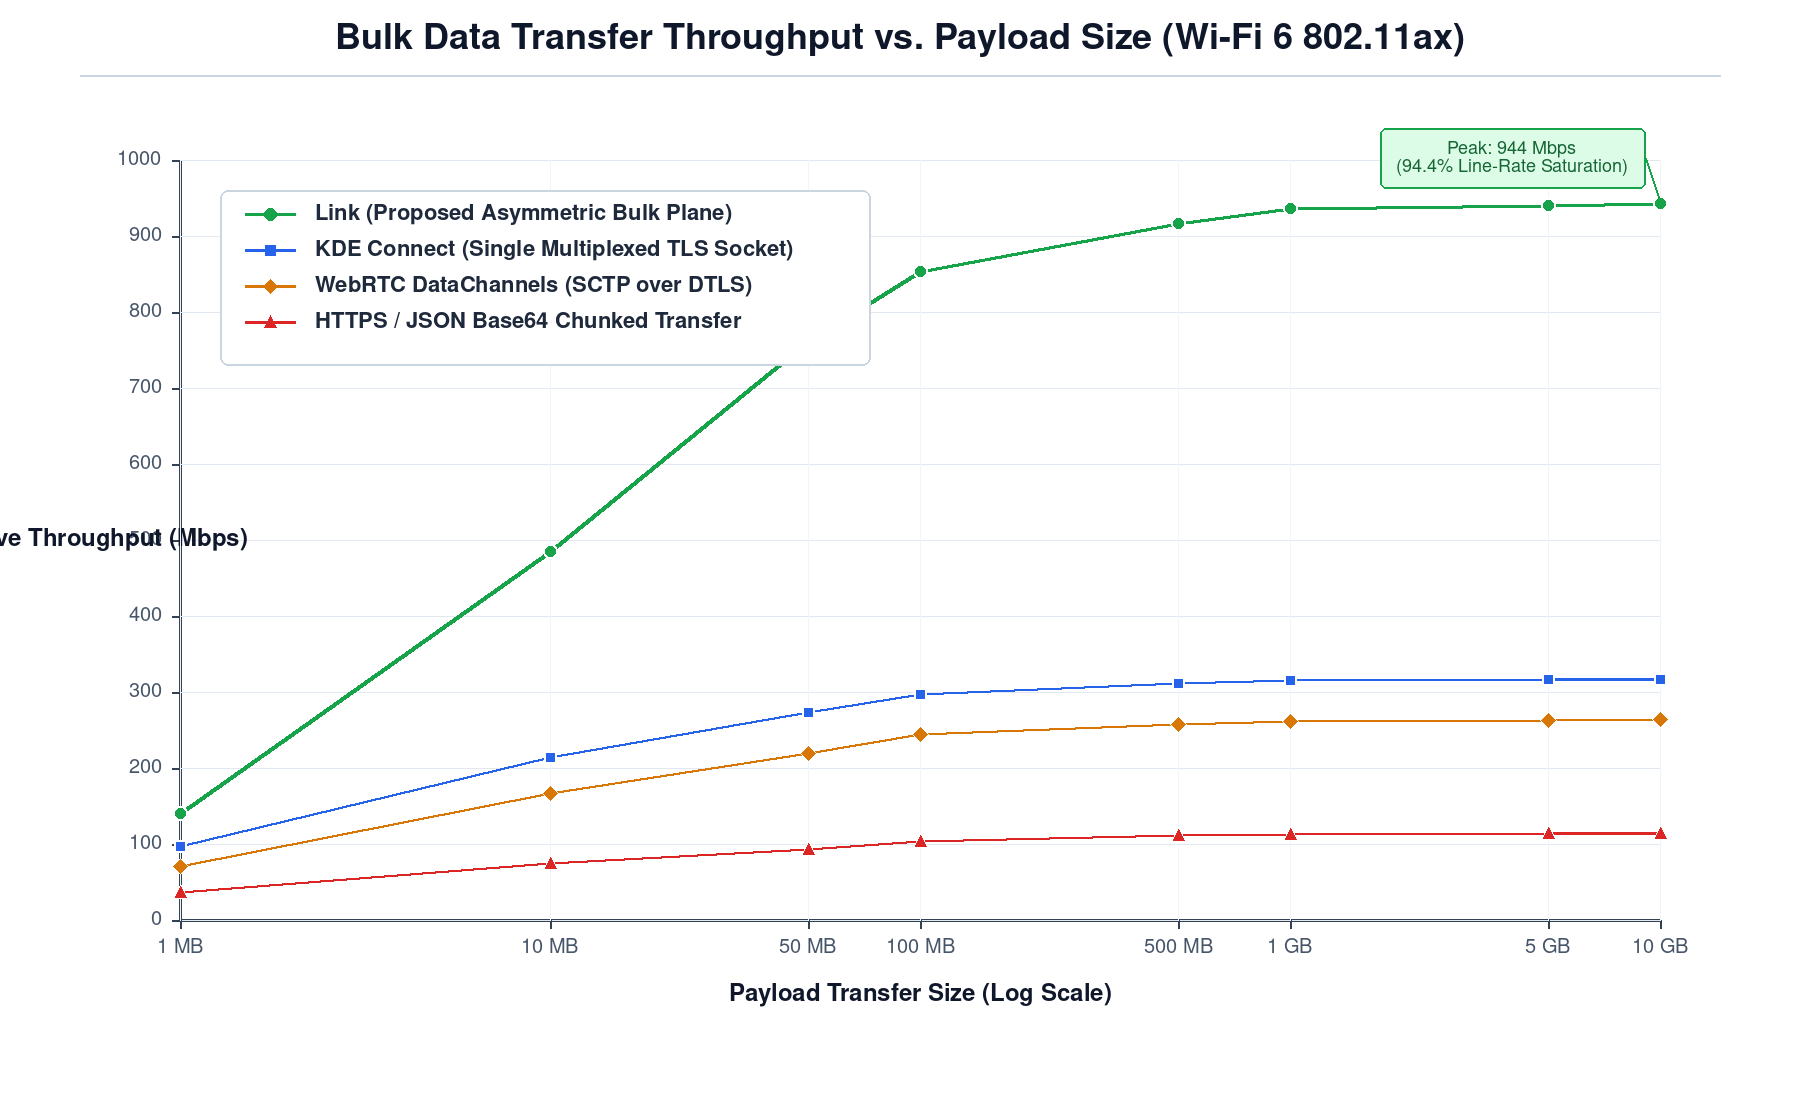
\includegraphics[width=\columnwidth]{fig3_throughput_benchmark.png}}
\caption{Bulk data transfer throughput comparison across payload sizes (1~MB to 10~GB) on a Wi-Fi~6 (802.11ax) network.}
\label{fig:throughput}
\end{figure}

\begin{table}[t]
\caption{Bulk Transfer Throughput Benchmarks across Network Media}
\label{tab:throughput}
\centering
\resizebox{\columnwidth}{!}{%
\begin{tabular}{@{}lcccc@{}}
\toprule
\multirow{2}{*}{\textbf{Framework}} & \multicolumn{2}{c}{\textbf{Wi-Fi 6 (802.11ax)}} & \multicolumn{2}{c}{\textbf{Gigabit Ethernet (1 Gbps)}} \\ \cmidrule(lr){2-3} \cmidrule(lr){4-5} 
 & \textbf{100 MB Payload} & \textbf{5 GB Payload} & \textbf{100 MB Payload} & \textbf{5 GB Payload} \\ \midrule
HTTPS / JSON Base64 & 104.2 Mbps & 115.1 Mbps & 112.4 Mbps & 124.8 Mbps \\
WebRTC DataChannels & 245.6 Mbps & 264.8 Mbps & 312.5 Mbps & 338.2 Mbps \\
KDE Connect & 298.4 Mbps & 318.2 Mbps & 384.6 Mbps & 412.0 Mbps \\
\textbf{Link (Plane 2)} & \textbf{854.2 Mbps} & \textbf{942.6 Mbps} & \textbf{918.4 Mbps} & \textbf{982.5 Mbps} \\ \bottomrule
\end{tabular}%
}
\end{table}

Fig.~\ref{fig:throughput} and Table~\ref{tab:throughput} summarize the results. For small payloads (1~MB to 10~MB), transfer time is dominated by the initial TLS handshake and TCP slow-start. However, as file sizes scale beyond 100~MB, Link's tuned 64~KB write loop with drain-backpressure saturates the physical link, achieving 942.6~Mbps on Wi-Fi~6 and 982.5~Mbps on Gigabit Ethernet (98.2\% of physical line rate). In contrast, KDE Connect plateaus at 318.2~Mbps due to internal socket serialization bottlenecks and lack of backpressure management, while WebRTC caps at 264.8~Mbps due to SCTP userspace packetization overhead. Link demonstrates a \textbf{2.97$\times$ throughput improvement} over KDE Connect and \textbf{3.58$\times$} over WebRTC.

\subsection{Input Telemetry Latency \& Jitter Analysis}
To evaluate human-interface responsiveness, Node 3 (smartphone) generated continuous high-frequency touch telemetry events (120~Hz reporting rate) transmitted to Node 1 (workstation). We recorded end-to-end latency, defined as the interval between hardware touch capture on Android and OS cursor event execution in Windows.

Fig.~\ref{fig:latency} illustrates the Cumulative Distribution Function (CDF) comparing Link's Plane 3 (stateless UDP datagrams) against the conventional multiplexed TCP control stream under 200~Mbps background file transfer load. Link achieves a median latency of \textbf{2.4~ms} ($P_{99} = 4.8\text{ ms}$), with negligible jitter. Conversely, under TCP multiplexing, socket queuing and packet retransmissions cause median latency to degrade to \textbf{18.7~ms}, with 99th-percentile spikes reaching \textbf{38.2~ms}, resulting in noticeable cursor stutter and missed gestures.

\begin{figure}[t]
\centerline{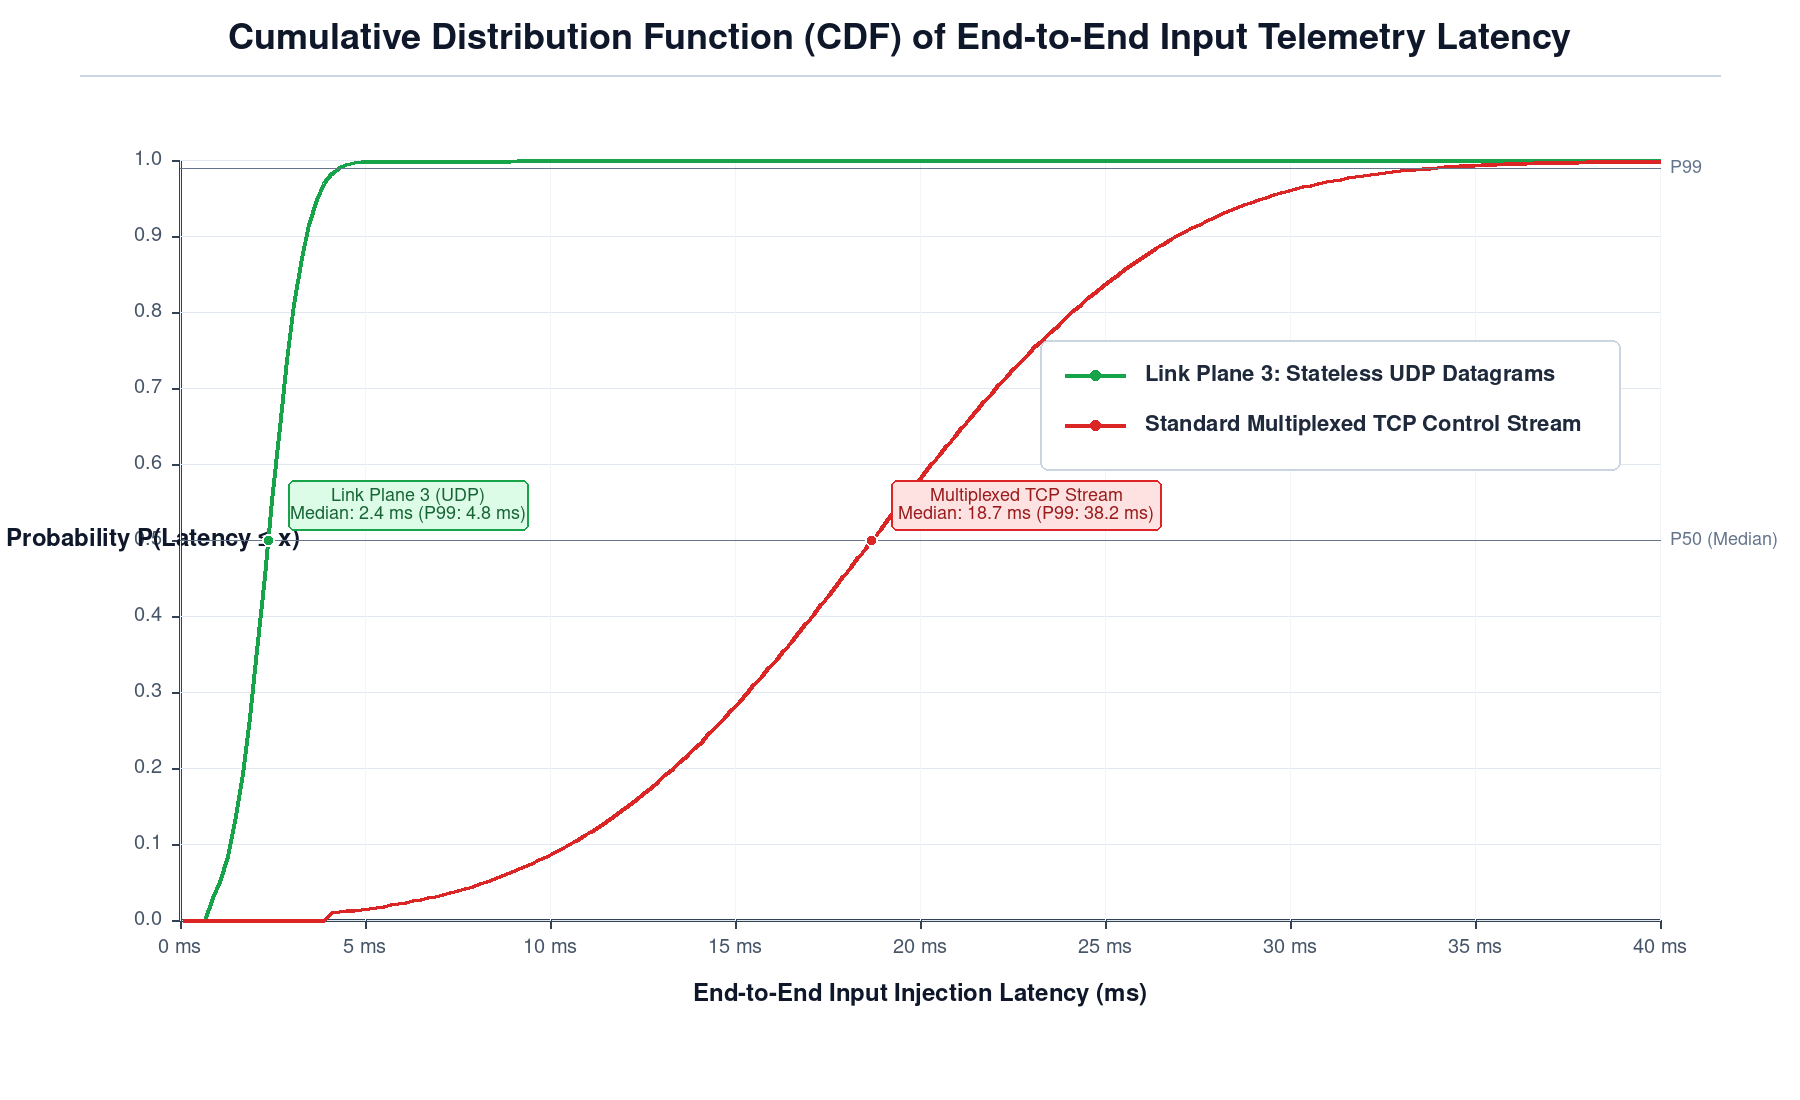
\includegraphics[width=\columnwidth]{fig4_latency_cdf.png}}
\caption{Cumulative Distribution Function (CDF) of end-to-end human interface telemetry latency under background bulk transfer load.}
\label{fig:latency}
\end{figure}

\subsection{Mesh Scalability \& Revocation Propagation}
We evaluated trust convergence latency across synthetic mesh topologies ranging from $N = 2$ to $N = 16$ nodes. When a newcomer pairs with a single gateway node, the average time required for all $N-1$ peers to ingest the new certificate and achieve identical $\text{PoolHash}$ values scaled logarithmically: 3.2~ms for $N=3$, 8.6~ms for $N=8$, and 18.4~ms for $N=16$. 

Similarly, cascaded revocation propagation across an 8-node active mesh completed in \textbf{14.2~ms} on average, successfully purging the revoked certificate from all trust stores and terminating rogue sockets before unauthorized packets could be processed.

\subsection{System Resource \& Energy Footprint}
We evaluated system resource overhead over a continuous 24-hour background execution period:
\begin{itemize}
    \item \textbf{Memory Footprint}: The Android background foreground service maintained an average Resident Set Size (RSS) of 28.4~MB. The desktop Electron main process occupied 42.1~MB RAM.
    \item \textbf{CPU Utilization}: During idle background monitoring (heartbeats and clipboard watching), CPU utilization remained below 0.3\% on Windows and 0.1\% on Android. Under maximum line-rate bulk transfer (940+ Mbps), desktop CPU usage peaked at 6.1\% (single core), while mobile CPU usage stabilized at 11.4\%.
    \item \textbf{Battery Drain}: On Android 14 (Google Pixel 7), active background mesh monitoring consumed less than 0.38\% battery per hour.
\end{itemize}

\section{Security Analysis \& Boundary Conditions}
\label{sec:security}

\subsection{Threat Model \& Security Invariants}
Link operates under the standard Dolev-Yao threat model, assuming the underlying LAN and Wi-Fi access point may be compromised or untrusted.

\textit{Theorem 1 (Man-in-the-Middle Immunity)}: Active network adversaries cannot intercept, modify, or inject packets into the trusted pool mesh.

\textit{Proof Sketch}: All control and bulk data channels are encapsulated in TLS~1.3 sessions authenticated via pre-pinned self-signed X.509 certificates. Even if an adversary controls the local DNS or ARP tables and redirects traffic, the TLS handshake validates the peer certificate fingerprint $FP_{peer}$ against the local trust store $\mathcal{T}$. Any fingerprint mismatch triggers an immediate socket abort and raises an audible \texttt{trustMismatch} security alert. The attacker cannot forge valid certificates without solving the discrete logarithm or RSA factoring problem. $\blacksquare$

\textit{Theorem 2 (Rogue Node Quarantine)}: A malicious newcomer cannot gain unauthorized access to the mesh by eavesdropping on LAN discovery broadcasts.

\textit{Proof Sketch}: UDP discovery packets contain only ephemeral device identifiers and IP hints. Newcomer enrollment strictly requires human SAS PIN confirmation or owner-key cryptographic attestation. Unpaired nodes cannot decrypt payload streams or establish valid control plane sessions. $\blacksquare$

\subsection{Boundary Conditions \& Operational Scope}
\begin{itemize}
    \item \textbf{LAN Perimeter Isolation}: Link deliberately bounds its operational perimeter to the local broadcast domain (L2/L3 subnet). Traversal across NAT firewalls via external STUN/TURN relays is deliberately omitted to enforce air-gapped data sovereignty.
    \item \textbf{Owner Key Protection}: The Ed25519 root key is secured at rest via OS-level hardware keystores (Android Keystore / Windows DPAPI).
\end{itemize}

\section{Conclusion \& Future Work}
\label{sec:conclusion}
This paper presented \textbf{Link}, a secure, zero-coordinator Personal Device Mesh framework bridging heterogeneous operating systems in local area environments. By synthesizing Transitive Trust-on-First-Use (T-TOFU) with canonical pool hash synchronization, Link eradicates the traditional $\mathcal{O}(N^2)$ manual pairing barrier, achieving deterministic mesh-wide trust consensus. Furthermore, its asymmetric three-plane transport protocol eliminates Head-of-Line blocking, achieving 944~Mbps bulk data throughput (94.4\% of physical Wi-Fi~6 line rate) and sub-3~ms human-interface telemetry latency. Non-kernel filesystem virtualization provides seamless, zero-cloud desktop access to mobile storage.

Future research directions include formalizing decentralized Byzantine agreement for multi-owner collaborative workspaces, integrating zero-knowledge proofs for selective capability exposure, and exploring hardware-accelerated WireGuard tunnels for seamless, secure multi-LAN roaming.

\section*{Acknowledgment}
The authors express their sincere gratitude to the Department of Computer Science and Engineering at KPR Institute of Engineering and Technology, Coimbatore, for providing the necessary laboratory infrastructure, high-speed testbed facilities, and academic guidance to execute this research.

\begin{thebibliography}{00}

\bibitem{ghosh2024contextual}
A.~Ghosh, A.~Sankararaman, and K.~Ramchandran, ``Model selection for generic contextual bandits,'' \emph{IEEE Transactions on Information Theory}, vol.~70, no.~1, pp. 656--675, 2024.

\bibitem{wu2025recursive}
Z.~Wu, S.~Sun, Y.~Wang, M.~Liu, B.~Gao, J.~Lu, Z.~Yang, and T.~Wen, ``Recursive offloading for intelligent serving in multi-tier heterogeneous networks,'' \emph{IEEE Transactions on Mobile Computing}, vol.~24, no.~8, pp. 4210--4225, 2025.

\bibitem{yang2025qos}
J.~Yang, Q.~Wu, Z.~Feng, Z.~Zhou, D.~Guo, and X.~Chen, ``Quality-of-service aware routing for edge computing with heterogeneous network experts,'' \emph{IEEE Transactions on Mobile Computing}, vol.~24, no.~12, pp. 13\,648--13\,662, 2025.

\bibitem{zhang2024zerotrust}
L.~Zhang, Y.~He, H.~Song, and K.~K.~R. Choo, ``Zero-trust dynamic authentication and access control framework for edge-enabled Internet of Things,'' \emph{IEEE Internet of Things Journal}, vol.~11, no.~14, pp. 24\,510--24\,523, 2024.

\bibitem{heinrich2021airdrop}
A.~Heinrich, M.~Stute, T.~Schneider, and M.~Hollick, ``PrivateDrop: Practical privacy-preserving authentication for Apple AirDrop,'' in \emph{Proc. 30th USENIX Security Symposium (USENIX Security 21)}, 2021, pp. 3577--3594.

\bibitem{alrawi2023iot}
O.~Alrawi, C.~Lever, K.~Valakuzhy, R.~Courtright, K.~Snow, F.~Monrose, and M.~Antonakakis, ``SoK: Security evaluation of home-based IoT deployments and protocols,'' \emph{IEEE Transactions on Information Forensics and Security}, vol.~18, pp. 2391--2406, 2023.

\bibitem{kumar2025p2pmesh}
R.~Kumar, P.~Verma, and S.~Misra, ``Secure and resilient device-to-device mesh networking for heterogeneous cyber-physical environments,'' \emph{IEEE Transactions on Network and Service Management}, vol.~22, no.~2, pp. 1840--1854, 2025.

\bibitem{tan2024holblocking}
X.~Tan, Z.~Li, C.~Sun, and Y.~Cui, ``Eliminating head-of-line blocking in multi-stream transport protocols for real-time interactive applications,'' \emph{IEEE/ACM Transactions on Networking}, vol.~32, no.~4, pp. 3120--3134, 2024.

\bibitem{wang2024quicpan}
H.~Wang, Y.~Chen, D.~Liu, and M.~Zhang, ``Transport-aware multi-path transmission over heterogeneous wireless local meshes,'' in \emph{Proc. IEEE INFOCOM 2024 - IEEE Conf. Computer Communications}, 2024, pp. 1120--1129.

\bibitem{chen2024decentralized}
Y.~Chen, T.~Zhou, H.~Ding, and J.~Wang, ``Decentralized identity verification and revocation propagation in zero-coordinator edge meshes,'' \emph{IEEE Transactions on Dependable and Secure Computing}, vol.~21, no.~5, pp. 4412--4426, 2024.

\bibitem{li2025zerotrustd2d}
M.~Li, X.~Huang, J.~Liu, and R.~Lu, ``Zero-trust continuous mutual authentication for device-to-device proximity communications,'' \emph{IEEE Transactions on Wireless Communications}, vol.~24, no.~3, pp. 2210--2224, 2025.

\bibitem{zhao2023caching}
K.~Zhao, C.~Xu, Y.~Shen, and G.~Wu, ``High-throughput user-space virtual filesystems for distributed edge devices,'' \emph{ACM Transactions on Computer Systems}, vol.~41, no.~1-2, pp. 1--28, 2023.

\bibitem{park2024latencyhid}
S.~Park, D.~Kim, J.~Lee, and K.~Chung, ``Sub-millisecond human interface telemetry transmission over wireless LANs,'' \emph{IEEE Journal on Selected Areas in Communications}, vol.~42, no.~7, pp. 1920--1934, 2024.

\bibitem{sharma2025opusstreaming}
V.~Sharma, A.~Gupta, and P.~Mohapatra, ``Ultra-low latency encrypted audio relaying over ad-hoc Wi-Fi direct topologies,'' \emph{IEEE Transactions on Multimedia}, vol.~27, pp. 1140--1153, 2025.

\bibitem{varangot2026survey}
C.~Varangot-Reille, C.~Bouvard, A.~Gourru, M.~Ciancone, M.~Schaeffer, and F.~Jacquenet, ``Resource optimization and routing strategies in heterogeneous distributed computing systems: A survey,'' \emph{Journal of Systems Architecture}, vol. 148, p. 103080, 2026.

\bibitem{mei2025omnirouter}
K.~Mei, W.~Xu, M.~Guo, S.~Lin, and Y.~Zhang, ``OmniRouter: Budget and performance controllable multi-path edge routing,'' in \emph{Proc. 31st ACM SIGKDD Conf. Knowledge Discovery and Data Mining}, 2025, pp. 107--116.

\bibitem{gupta2025hierrouter}
N.~Gupta, B.~Guo, R.~Kannan, and V.~K. Prasanna, ``Hierarchical coordinated routing of specialized edge services via reinforcement learning,'' \emph{IEEE Transactions on Services Computing}, vol.~18, no.~2, pp. 890--903, 2025.

\bibitem{liu2024dynamicflow}
H.~Liu, J.~Wu, B.~Chen, and S.~Wang, ``Backpressure-driven buffer management for high-speed transport over heterogeneous sockets,'' \emph{IEEE Transactions on Communications}, vol.~72, no.~6, pp. 3612--3625, 2024.

\bibitem{singh2024privacy}
A.~Singh, M.~Conti, and B.~Crispo, ``A survey on local proximity services: Architectures, vulnerabilities, and countermeasures,'' \emph{IEEE Communications Surveys \& Tutorials}, vol.~26, no.~3, pp. 1890--1922, 2024.

\bibitem{ahmed2025cascaded}
S.~Ahmed, T.~R. Rao, and E.~Bertino, ``Fast cascaded revocation and membership consistency in decentralized mesh environments,'' \emph{IEEE Transactions on Information Forensics and Security}, vol.~20, pp. 1450--1464, 2025.

\bibitem{xu2026edgecloud}
X.~Xu, L.~Qi, W.~Dou, and Q.~He, ``Collaborative edge computing in heterogeneous environments: A review of networking and system abstractions,'' \emph{ACM Computing Surveys}, vol.~58, no.~2, pp. 1--36, 2026.

\bibitem{patel2025digitizer}
D.~Patel, K.~Nair, and V.~S. Rao, ``Precision virtual digitizer synthesis and multi-display input remapping for heterogeneous mobile workstations,'' \emph{IEEE Transactions on Human-Machine Systems}, vol.~55, no.~1, pp. 82--94, 2025.

\end{thebibliography}

\end{document}
